\documentclass[a4paper,10pt]{article}
\usepackage[utf8]{inputenc}
\usepackage{graphicx}



%opening
\title{Simulaci\'on de la poblacion de la ESCOM a diferentes actividades}
\author{Jonathan Arcos Ayala}
\date{Julio, 2015}

\begin{document}

\maketitle

\newpage

\section{Introducci\'on}

En el estudio de los sistemas complejos podemos ver que uno de los grandes problemas es poder extraer todas las caracter\'isticas del sistema y hacer un aut\'omata celular que nos d\'e el comportamiento del sistema en cualquier caso. 
\\ \\
Esta manera de modelar es muy eficiente pero requiere de muchos recursos computacionales para representar el comportamiento del sistema, y es casi imposible hacerlo cuando se tiene un universo demasiado grande, ya que el n\'umero de estados de nuestro aut\'omata crecen exponencialmente.
\\ \\
Otra manera de poder visualizar el comportamiento de los sistemas complejos es por medio de las simulaciones, ya que estas nos van describiendo el comportamiento que puede tener el sistema con forme transcurre el tiempo.
\\ \\
La simulaci\'on de los sistemas complejos es una de las t\'ecnicas m\'as utilizadas, y por ello este m\'etodo se ha diversificado de tal manera que hoy en d\'ia podemos encontrar t\'ecnicas, como la de agentes, que se especializan en el an\'alisis de un tipo de situaciones en un sistema complejo. 
\\ \\
La t\'ecnica de simulaci\'on por agentes se basa en generar diferentes grupos de la poblaci\'on y a cada grupo generarle un perfil, as\'i en lugar de tener que describir el comportamiento de cada una persona en la poblaci\'on solo se describe el comportamiento de los grupos de generados. Esto hace que al momento de la simulaci\'on la complejidad sea menor y podamos entregar un comportamiento bastante parecido al que se tendr\'ia en la realidad.
\\ \\
En este documento veremos la implementaci\'on de una t\'ecnica de agentes en la simulaci\'on del comportamiento de la poblaci\'on de la escuela superior de c\'omputo dentro de las instalaciones y sus alrededores. Para ello utilizaremos un simulador de agentes llamada “Pedestrian Dynamics Trial”, para construir a groso modo las instalaciones de la Escuela Superior de C\'omputo (ESCOM) y sus alrededores, adem\'as de describir el comportamiento de los alumnos y profesores de la misma.


\section{Desarrollo de la simulaci\'on.}
\subsection{Ambiente de la simulaci\'on.}

Para iniciar la simulaci\'on primero fue necesario hacer un plano de las instalaciones de la escuela superior de computo con los lugares m\'as representativos, a continuaci\'on tenemos la descripci\'on del plano echo para la simulaci\'on.
\\ \\
Lo primero que hicimos fue generar un bosquejo de las instalaciones y los alrededores de la ESCOM, en este bosquejo se tomaron a los edificios, rejas, jardineras y la plancha de astas banderas como si fueran obst\'aculos ya que la poblaci\'on no puede atravesarlos de un lado al otro.
\\ \\
Para representar los salones, cub\'iculos, espacios de recreaci\'on y talleres fueron representadas por \'areas de estar, ya que la mayor\'ia la poblaci\'on podr\'ia estar en estos lugares desarrollando diferentes actividades sin la necesidad de salir de estas \'areas.
\\ \\
Las cafeter\'ias cercanas a la escuela, incluyendo la cafeter\'ia de la escuela, y algunas de las tiendas de conveniencia cercanas son representadas por \'areas de comercio en nuestro simulador, tambi\'en d\'andoles una caracter\'istica extra de retener a los agentes que llegan por un m\'inimo de tiempo de 15 min.
\\ \\
Las entradas que tiene la escuela son t\'ecnicamente 2, la entrada que est\'a cercana a la estaci\'on del metro polit\'ecnico y la segunda es la entrada que est\'a a espaldas de la plaza comercial Torres Lindavista, estas 2 entradas fueron representadas por 2 \'areas de generaci\'on de agentes, las cuales simularan la entrada y salida de la poblaci\'on de la escuela superior de computo.
\\ \\
Por ultimo podremos visualizar unos recuadros con alarmas del lado izquierdo de las instalaciones de la ESCOM, las cuales se van activando para que los agentes realicen diferentes tareas dentro de las instalaciones de la escuela.
\\ \\
Todo lo descrito en la parte de arriba lo podemos visualizar en la siguiente imagen.
\\ \\

%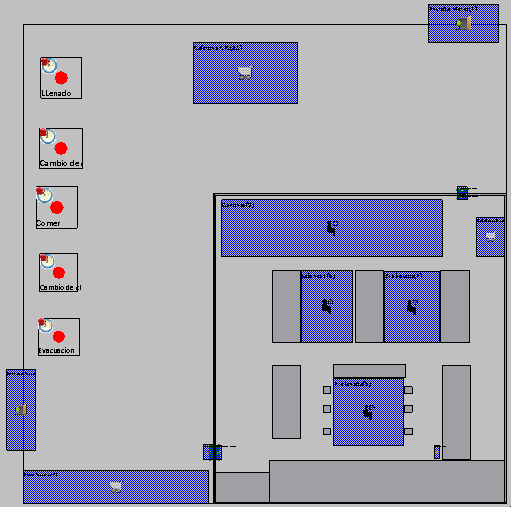
\includegraphics{M1.png}
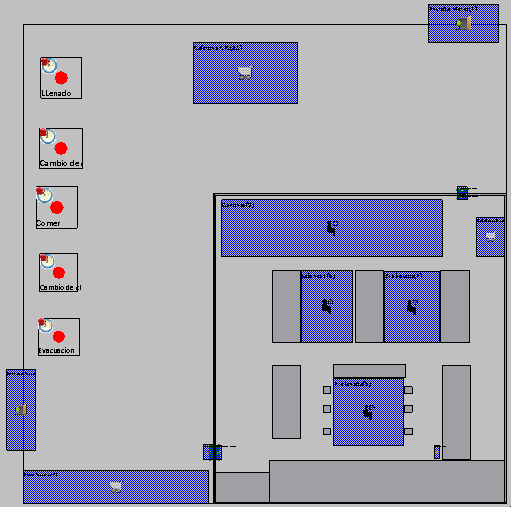
\includegraphics{M1}

\\

\subsection{Generaci\'on de actividades}

Una vez que tenemos en el plano todos los elementos principales que constituyen a la ESCOM seguiremos con la descripci\'on de los perfiles que tendr\'an los agentes que vivir\'an en nuestra simulaci\'on. 
\\ \\ 
Los grupos de la poblaci\'on que se les genero un perfil para esta simulaci\'on fueron a los alumnos, ya que representan el grueso de la poblaci\'on de la ESCOM, y los profesores porque ellos tambi\'en representan una parte de la poblaci\'on importante en la escuela.
\\ \\
Una vez que identificamos los grupos de la poblaci\'on que participaran en esta simulaci\'on procedimos a generar las actividades que pueden realizar los agentes, estas actividades fueron las siguientes:
\\ \\

\begin{enumerate}
 \item[Entry:]Esta actividad representa la entrada de los agentes al sistema que en nuestro caso representa la entrada de los profesores y alumnos.
 \item[Exit:]Esta actividad se refuere a la salida de los agentes del sistema que en nuestro caso representa cuando un profesor o alumnos se retira de la escuela.
 \item[Tomar clases:]Esta actividad representa la entrada de los alumnos y profesores a  las aulas de clase.
 \item[Checar Entrada:]Esta actividad es exclusiva del agente profesor ya que el si tiene que reportar su entrada y su salida.
 \item[Comer:]En esta actividad participan los 2 agentes del sistema y representan la salida de las instalaciones de la ESCOM para ir alguna de las cafeter\'ias o a las tiendas de conveniencias de la plaza torres.
 \item[Emergency Exit:]Esta es una actividad especial parecida a la Actividad de Exit, la diferencia es que este si es un desalojo total de las instalaciones.
 \item[Entrada a la escuela:]Esta actividad representa la entrada de los agentes de los alrededores de la escuela a los edificios.
 \item[Esparcimiento:]Esta actividad representa cuando los agentes no tienen una actividad fija en las instalaciones de la ESCOM.

\end{enumerate}

En la vida real lo poblaci\'on no tiene a realizar todas estas actividades al mismo tiempo y as\'i los mismos lugares, por esta raz\'on las actividades descritas anteriormente en la simulaci\'on tienen una regla probabil\'istica de si el agente realizara o no una actividad y si se realizara la actividad en que espacio de la ESCOM el agente realizara esta actividad.
\\ \\
A continuaci\'on daremos la descripci\'on de las reglas que rigen a cada actividad descrita previamente:

\begin{enumerate}
 \item[Entry:]La generaci\'on de agentes est\'a dada por una distribuci\'on uniforme en cada una de las 2 entradas propuestas en el esquema. Esta distribuci\'on tiene la siguiente formula:
\\ \\
Uniforme (2,15)
\\ \\
Donde: 
\begin{itemize}
 \item U representa una distribuci\'on de probabilidad uniforme.
 \item 2 representa el valor m\'inimo para la distribuci\'on uniforme.
 \item 15 representa el valor m\'aximo para la distribuci\'on uniforme
\end{itemize}

El par\'ametro de valor m\'aximo puede variar en los valores de 15, 20 y 25 para dar una densidad poblacional de 250, 400 y 800 aproximadamente.
\\ \\

 
 \item[Exit:]La salida de los agentes est\'a dada por una probabilidad uniforme a cada una de las 2 salidas propuestas en el esquema. Esta probabilidad est\'a distribuida por la siguiente formula:

\begin{itemize}
 \item Salida Metro = 50\%
 \item Salida Torres = 50\%
\end{itemize}

 \item[Tomar clases:]Esta actividad tiene una probabilidad uniforme a cada una de las 4 \'areas de estar que se tienen representadas en el esquema. Esta probabilidad est\'a distribuida por la siguiente formula:

\begin{itemize}
 \item Explanada = 20\%

 \item Salones = 35\%

 \item Biblioteca = 40\%

 \item Canchas = 5\%
 
\end{itemize}

 \item[Checar Entrada:]Esta actividad tiene una probabilidad uniforme del 100\% para los profesores y una probabilidad de 0\% para los alumnos para ir al \'area de checar.
 \item[Comer:]La actividad de comer tiene una probabilidad uniforme entre las 3 \'areas de comercio. Esta probabilidad est\'a distribuida con la siguiente formula:
\begin{itemize}
 \item CIC = 10\%

 \item Plaza Torres = 50\%

 \item Cafeter\'ia ESCOM = 10\% 
\end{itemize}


 \item[Emergency Exit:]En esta actividad desaloja a los agentes del sistema bajo una distribuci\'on uniforme. 
 \item[Entrada a la escuela:]Esta actividad tiene una probabilidad uniforme a cada una de las 2 entradas a las instalaciones de la escuela. Esta probabilidad est\'a distribuida  por la siguiente formula:

\begin{itemize}
 \item Entrada Torres = 70\%

 \item Entrada Metro = 30\% 
\end{itemize}


 \item[Esparcimiento:]Esta actividad tiene una probabilidad uniforme en cada unad de las 4 \'areas de estar. Esta probabilidad est\'a distribuida por la siguiente formula:

\begin{itemize}
 \item Explanada = 5%

 \item Salones = 2%

 \item Biblioteca = 2%

 \item Canchas = 15%
 
 \end{itemize}

\end{enumerate}

\subsection{Generaci\'on de perfiles}

Para terminar de los perfiles de los agente es necesario darles una secuencia de actividades que tienen que hacer los agentes. Estas listas de actividades van a ser activadas dependiendo del tiempo transcurrido en el sistema y las alarmas que se vayan activando. En la siguiente imagen se ver\'an las listas de actividades que fueron utilizadas en esta simulaci\'on.
\\ \\
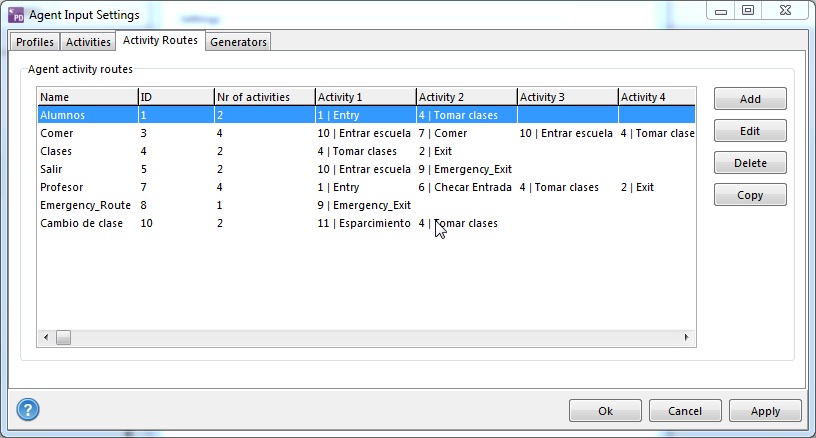
\includegraphics{M2}
\\ \\
Para poder iniciar ya la simulaci\'on se necesita que los agentes puedan desplazarse por el entorno dise\~nado para cumplir con el listado de actividades propuesto previamente, para ello es necesario

\section{Experimento}

Los experimentos que se hicieron fueron probar la secuencia de alarmas (llenado, Cambio de clases, Comer, Cambio de clases, Evacuaci\'on) con diferentes densidades de agentes dentro del sistema para ver el comportamiento de las masas de agentes en las entradas a los edificios de ESCOM.
\\ \\
El primer experimento realizado fue con una densidad aproximada de 250 agentes dentro del sistema, los cuales siguieron la secuencia de alarmas programadas:

\begin{enumerate}
 \item[Llenado:]El sistema arranca llenado el sistema con agentes que entran  desde las 2 entradas propuestas durante 10 min.

 \item[Cambio de clase:]Esta alarma genera un reacomodo de los agentes en las 4 \'areas de estar, esta alarma se activa cuando haya transcurrido 8:30:00 hrs.

 \item[Comer:]Cuando el sistema lleva transcurridas 10:30:00 hrs dispara una alarma que ejecuta las acciones de todos los agentes a moverse a las \'areas de comercio.

 \item[Cambio de clase:]Esta alarma genera un reacomodo de los agentes en las 4 \'areas de estar, esta alarma se activa cuando haya transcurrido 12:00:00 hrs.

 \item[Evacuaci\'on:]Esta alarma genera una evacuaci\'on masiva de todos los agentes del sistema.

\end{enumerate}

Esta misma secuencia de alarmas fue ejecutada para poblaciones  con una densidad de 400 agentes y 800 agentes aproximadamente.

\newpage

\section{Conclusiones.}

En esta pr\'actica vimos como es el comportamiento general de la poblaci\'on de la ESCOM ante ciertos acontecimientos cotidianos como el salir a comer o cambiar de clase, las cuales se ven el comportamiento probable de alumnos y profesores dentro de las instalaciones. Este comportamiento de los agentes nos dice que no existe una gran complicaci\'on en el desplazamiento de los alumnos y profesores dentro de las instalaciones de la escuela si la densidad de la poblaci\'on es baja; con forme la densidad de poblaci\'on incrementa se ve un tr\'afico en los pasillos.
\\ \\
Otro fen\'omeno que podemos observar en la simulaci\'on es cuando generamos una alarma de emergencia para todos los agentes, los cuales tienen que salir del sistema lo m\'as r\'apido posible. Lo que se observo fue que las salidas de la escuela no son suficientes para desalojar a toda la poblaci\'on inmediatamente ya que desde una densidad de 250 agentes aproximadamente se ve un embotellamiento de agentes en las entradas a las instalaciones de la escuela. La \'unica diferencia que vemos dependiendo de la densidad que se programe en el sistema es el tiempo que tanda en desalojar a la poblaci\'on variando desde los 2 minutos hasta los 20 minutos.
\\ \\
Por lo tanto vemos que las entradas de la escuela no son tan eficientes al momento de desalojar a la poblaci\'on total en caso de una emergencia o contingencia. 
\\
\end{document}
